\documentclass[12pt]{article}
\usepackage{../preamble3}
%\pagenumbering{gobble}
\title{MathCounts Chapter Invitational February 2021 \\ Target Round}
\author{Patrick \& James Toche}
\date{Revised:~\today}

\begin{document}
\maketitle
\begin{minipage}{\textwidth}
\begin{abstract}\setlength{\parindent}{0pt}%
Notes on Target Round of MathCounts Invitational Competition, February 2021. 
Questions are from MathCounts Foundation (\url{https://www.mathcounts.org/}). Copyright restrictions may apply. Written for personal use. 
Please report typos and errors over at \url{https://github.com/ptoche/Math/tree/master/mathcounts}. 
\end{abstract}
\end{minipage}

\thispagestyle{empty}
\clearpage
\addtocounter{page}{-1}

\section*{Target Round}


%%%%%%%%%%%%%%%%%%%%%%%%%%%%%%%%%%%%%%%%%%%%%%%%%%%%%%%%%%%%%%%%%%%%%%%%
\subsection*{1.}
Max is buying hot dogs and buns for dinner. If hot dogs are sold in packages of six and buns are sold in packages of eight, what is the least positive number of hot dogs that Max must buy so that he can purchase exactly the same number of buns? 

\fbox{\phantom{ANSWER}}~hot dogs

\begin{answer}
\begin{tikzpicture}\node[textbox]{%
    \begin{minipagex}{\dimexpr\textwidth-20pt}
        The least common multiple of $6$ and $8$ can be found with one of these approaches: 
        \begin{enumerate}
        \item list multiples of $6$ until one of them is a multiple of $8$.
        \item list multiples of $8$ until one of them is a multiple of $6$.
        \end{enumerate}
        The second approach would be a little quicker. We have $8$, $16$, $24$, stop.
        \begin{empheq}[box={\mathbox[colback=white]}]{equation*}
            24 ~\text{hot dogs}
        \end{empheq} 
    \end{minipagex}
    };
\end{tikzpicture}%
\end{answer}
%%%%%%%%%%%%%%%%%%%%%%%%%%%%%%%%%%%%%%%%%%%%%%%%%%%%%%%%%%%%%%%%%%%%%%%%


%%%%%%%%%%%%%%%%%%%%%%%%%%%%%%%%%%%%%%%%%%%%%%%%%%%%%%%%%%%%%%%%%%%%%%%%
\subsection*{2.}
The square card shown in Figure~A, with area $16$ units$^2$, is folded twice along the dashed lines to get the square shown in Figure~B. Then, scissors are used to cut through the folded square, and one-fourth of the folded card, shown shaded in Figure~C, is removed. When unfolded, what is the area of what remains of the card after the removal? 

\begin{minipagex}[b]{\linewidth}
\centering
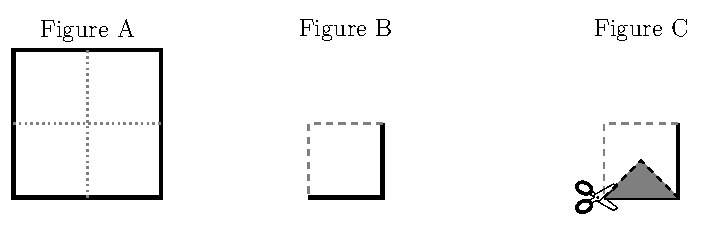
\includegraphics[height=6cm]{target-02-figure}
\end{minipagex}

\nopagebreak

\fbox{\phantom{ANSWER}}~units$^2$

\begin{answer}
\begin{tikzpicture}\node[textbox]{%
    \begin{minipagex}{\dimexpr\textwidth-20pt}
        The area removed by one triangular cut is equal to one-fourth of one-fourth of the large square in Figure~A. Because of the folding, there are four such triangular cuts, so that the total area removed is one-fourth of the area of the large square, or $16/4=4$. The area of what remains is therefore $16-4=12$. 
        \begin{empheq}[box={\mathbox[colback=white]}]{equation*}
            12 ~\text{units}^2
        \end{empheq} 
    \end{minipagex}
    };
\end{tikzpicture}%
\end{answer}
%%%%%%%%%%%%%%%%%%%%%%%%%%%%%%%%%%%%%%%%%%%%%%%%%%%%%%%%%%%%%%%%%%%%%%%%


%%%%%%%%%%%%%%%%%%%%%%%%%%%%%%%%%%%%%%%%%%%%%%%%%%%%%%%%%%%%%%%%%%%%%%%%
\subsection*{3.}
Cindy has been given four chores to complete today: vacuum, mop, dust and laundry. Because Cindy finds doing laundry especially unpleasant, she wants to do that chore last. Given this, in how many different orders can Cindy complete her chores? 

\nopagebreak

\fbox{\phantom{ANSWER}}~orders

\begin{answer}
\begin{tikzpicture}\node[textbox]{%
    \begin{minipagex}{\dimexpr\textwidth-20pt}
        One of the $4$ objects has its position predetermined (laundry), so that we are looking for the number of ways to permute $3$ objects.
        \begin{align*}
        3! = 3 \times 2 = 6
        \end{align*}
        \begin{empheq}[box={\mathbox[colback=white]}]{equation*}
            6 ~\text{orders}
        \end{empheq} 
    \end{minipagex}
    };
\end{tikzpicture}%
\end{answer}
%%%%%%%%%%%%%%%%%%%%%%%%%%%%%%%%%%%%%%%%%%%%%%%%%%%%%%%%%%%%%%%%%%%%%%%%


%%%%%%%%%%%%%%%%%%%%%%%%%%%%%%%%%%%%%%%%%%%%%%%%%%%%%%%%%%%%%%%%%%%%%%%%
\subsection*{4.}
In the dice game Zero, a player rolls six standard six-sided dice and then scores points for certain combinations, as shown in the table. A die cannot be used in more than one combination. For example, a player who rolls $1$~$5$~$6$~$4$~$4$~$6$ scores $50$ points, while a player who rolls $1$~$4$~$4$~$4$~$1$~$4$ scores $250$ points. What is the probability that a player scores $0$ points on a roll? Express your answer as a common fraction. 

\begin{center}
  \rowcolors{1}{white}{gray!20}
\begin{tabular}{L{6cm}R{3cm}} 
\toprule
  Player's Roll & Points Scored \\
\midrule
  Three of a kind (ex. $2$~$2$~$2$~$4$~$6$~$3$) & 100 \\
  Four of a kind                                & 200 \\
  Five of a kind                                & 400 \\
  Six of a kind                                 & 900 \\
  Three pairs (ex. $2$~$2$~$3$~$3$~$4$~$4$)     & 200 \\
  Six distinct (ex. $1$~$2$~$3$~$4$~$5$~$6$)    & 300 \\
  The number $1$                                &  25 \\
  The number $5$                                &  25 \\
\bottomrule
\end{tabular}
\end{center}

\nopagebreak

\begin{minipage}[b]{\linewidth}
\fbox{\phantom{ANSWER}}\\
\mbox{---------------}\\
\fbox{\phantom{ANSWER}}
\end{minipage}


\begin{answer}
\begin{tikzpicture}\node[textbox]{%
    \begin{minipagex}{\dimexpr\textwidth-20pt}
        The configurations that yield no points are $2$~$3$~$4$~$6$ with two numbers repeated but no triple. The number of ways to choose $2$ objects from $6$ is 
        \begin{align*}
        \comb{2}{6} = \frac{6!}{2!(6-2)!} = \frac{6 \times 5}{2} = 15
        \end{align*}
        To properly calculate the probability, we also need to take into account permutations of these six rolls ($6!$).
        The number of ways to roll six six-sided dice is $6^6$. 
        Thus, the probability is the ratio of these:
        \begin{align*}
        \frac{15 \times 6!}{6^6} 
          = \frac{5}{216}
        \end{align*}
        \begin{empheq}[box={\mathbox[colback=white]}]{equation*}
            \frac{5}{216}
        \end{empheq} 
    \end{minipagex}
    };
\end{tikzpicture}%
\end{answer}
%%%%%%%%%%%%%%%%%%%%%%%%%%%%%%%%%%%%%%%%%%%%%%%%%%%%%%%%%%%%%%%%%%%%%%%%


%%%%%%%%%%%%%%%%%%%%%%%%%%%%%%%%%%%%%%%%%%%%%%%%%%%%%%%%%%%%%%%%%%%%%%%%
\subsection*{5.}
A U.S. quarter is $0.069$ inches thick. Clayton Kershaw earned $33$ million dollars for the $2017$ Major League Baseball season. If Kershaw received his entire $2017$ salary in the form of a single stack of quarters, what would be the height of the stack, in miles? There are $5280$ feet in a mile. Express your answer as a decimal to the nearest hundredth. 

\nopagebreak

\fbox{\phantom{ANSWER}}~units$^2$

\begin{answer}
\begin{tikzpicture}\node[textbox]{%
    \begin{minipagex}{\dimexpr\textwidth-20pt}
        A dollar in quarters is 
        \begin{align*}
        4 \times 0.069 = 0.276 ~\text{inches}
        \end{align*}
        $33$ million of those is 
        \begin{align*}
        33 \times 0.276 = 9,108,000 ~\text{inches}
        \end{align*}
        Converted to feet:
        \begin{align*}
        9,108,000~\text{inches} \times \frac{1~\text{foot}}{12~\text{inches}} = 759,000~\text{feet}
        \end{align*}
        Converted to miles:
        \begin{align*}
        759,000~\text{feet} \times \frac{1~\text{mile}}{5280~\text{feet}}
         = 143.75~\text{miles} 
        \end{align*}
        \begin{empheq}[box={\mathbox[colback=white]}]{equation*}
            143.75~\text{miles} 
        \end{empheq} 
    \end{minipagex}
    };
\end{tikzpicture}%
\end{answer}
%%%%%%%%%%%%%%%%%%%%%%%%%%%%%%%%%%%%%%%%%%%%%%%%%%%%%%%%%%%%%%%%%%%%%%%%



%%%%%%%%%%%%%%%%%%%%%%%%%%%%%%%%%%%%%%%%%%%%%%%%%%%%%%%%%%%%%%%%%%%%%%%%
\subsection*{6.}
In rectangle $ABCD$ the length of side $AB$ is less than the length of side $BC$. When diagonal $AC$ is drawn, and a line segment from vertex $B$ to diagonal $AC$ is drawn so that the segment meets $AC$ at a right angle, rectangle $ABCD$ is divided into three regions whose areas form an arithmetic progression. The ratio $AB{:}BC$, expressed as a common fraction in simplest radical form is $\dfrac{\sqrt{a}}{b}$. What is the value of $ab$? 

\nopagebreak

\fbox{\phantom{ANSWER}}

\begin{answer}
\begin{tikzpicture}\node[textbox]{%
    \begin{minipagex}{\dimexpr\textwidth-20pt}
        TO DO: COPY MY NOTES
        Applying the Pythagorean theorem,
        \begin{align*}
        = \sqrt{\frac{1}{2}} 
          = \frac{1}{\sqrt{2}}
          \frac{\sqrt{2}}{2} 
        \end{align*}
        It follows that
        \begin{align*}
        \frac{\sqrt{a}}{b} = \frac{\sqrt{2}}{2} 
        \Rightarrow
          a = b = 2 
        \Rightarrow 
          ab = 4
        \end{align*}
        \begin{empheq}[box={\mathbox[colback=white]}]{equation*}
            4
        \end{empheq} 
    \end{minipagex}
    };
\end{tikzpicture}%
\end{answer}
%%%%%%%%%%%%%%%%%%%%%%%%%%%%%%%%%%%%%%%%%%%%%%%%%%%%%%%%%%%%%%%%%%%%%%%%


%%%%%%%%%%%%%%%%%%%%%%%%%%%%%%%%%%%%%%%%%%%%%%%%%%%%%%%%%%%%%%%%%%%%%%%%
\subsection*{7.}
If C is the temperature in degrees Celsius, the temperature in degrees Farenheit is given by the formula $\text{F}=\dfrac{9}{5}\text{C}+32$. On a cold winter day, the temperature in degrees Farenheit is the additive inverse of the temperature in degrees Celsius. What is the temperature in degrees Celsius? Express your answer as a decimal to the nearest tenth. 

\nopagebreak

\fbox{\phantom{ANSWER}}~$^{\circ}$C

\begin{answer}
\begin{tikzpicture}\node[textbox]{%
    \begin{minipagex}{\dimexpr\textwidth-20pt}
        The main difficulty here is knowing that the ``additive inverse'' of $x$ is the number $y$ such that $x+y=0$, in other words the additive inverse of $x$ is $-x$, its ``opposite.'' The verbal statement yields a system of two equations in two unknowns:
        \begin{align*}
        \text{F} & = \dfrac{9}{5}\text{C} + 32 \\
        \text{F} & = -\text{C}
        \end{align*}
        which may be solved by substitution:
        \begin{align*}
        -\text{C} = \dfrac{9}{5}\text{C} + 32 
        \Rightarrow
        \left(\frac{9}{5}+1\right) \text{C} 
                  = -32 
        \Rightarrow
         \text{C} = -32 \times \frac{5}{14} 
                  \approx -11.429
        \end{align*}
        \begin{empheq}[box={\mathbox[colback=white]}]{equation*}
            -11.4~^{\circ}\text{C}
        \end{empheq} 
    \end{minipagex}
    };
\end{tikzpicture}%
\end{answer}
%%%%%%%%%%%%%%%%%%%%%%%%%%%%%%%%%%%%%%%%%%%%%%%%%%%%%%%%%%%%%%%%%%%%%%%%



%%%%%%%%%%%%%%%%%%%%%%%%%%%%%%%%%%%%%%%%%%%%%%%%%%%%%%%%%%%%%%%%%%%%%%%%
\subsection*{8.}
How many ways are there to color the $4 \times 4$ grid shown, so that each unit square is red, blue, green, or yellow, and so that each square is the same color as exactly two of the squares that share a side with it?

\begin{minipagex}[b]{\linewidth}
\centering
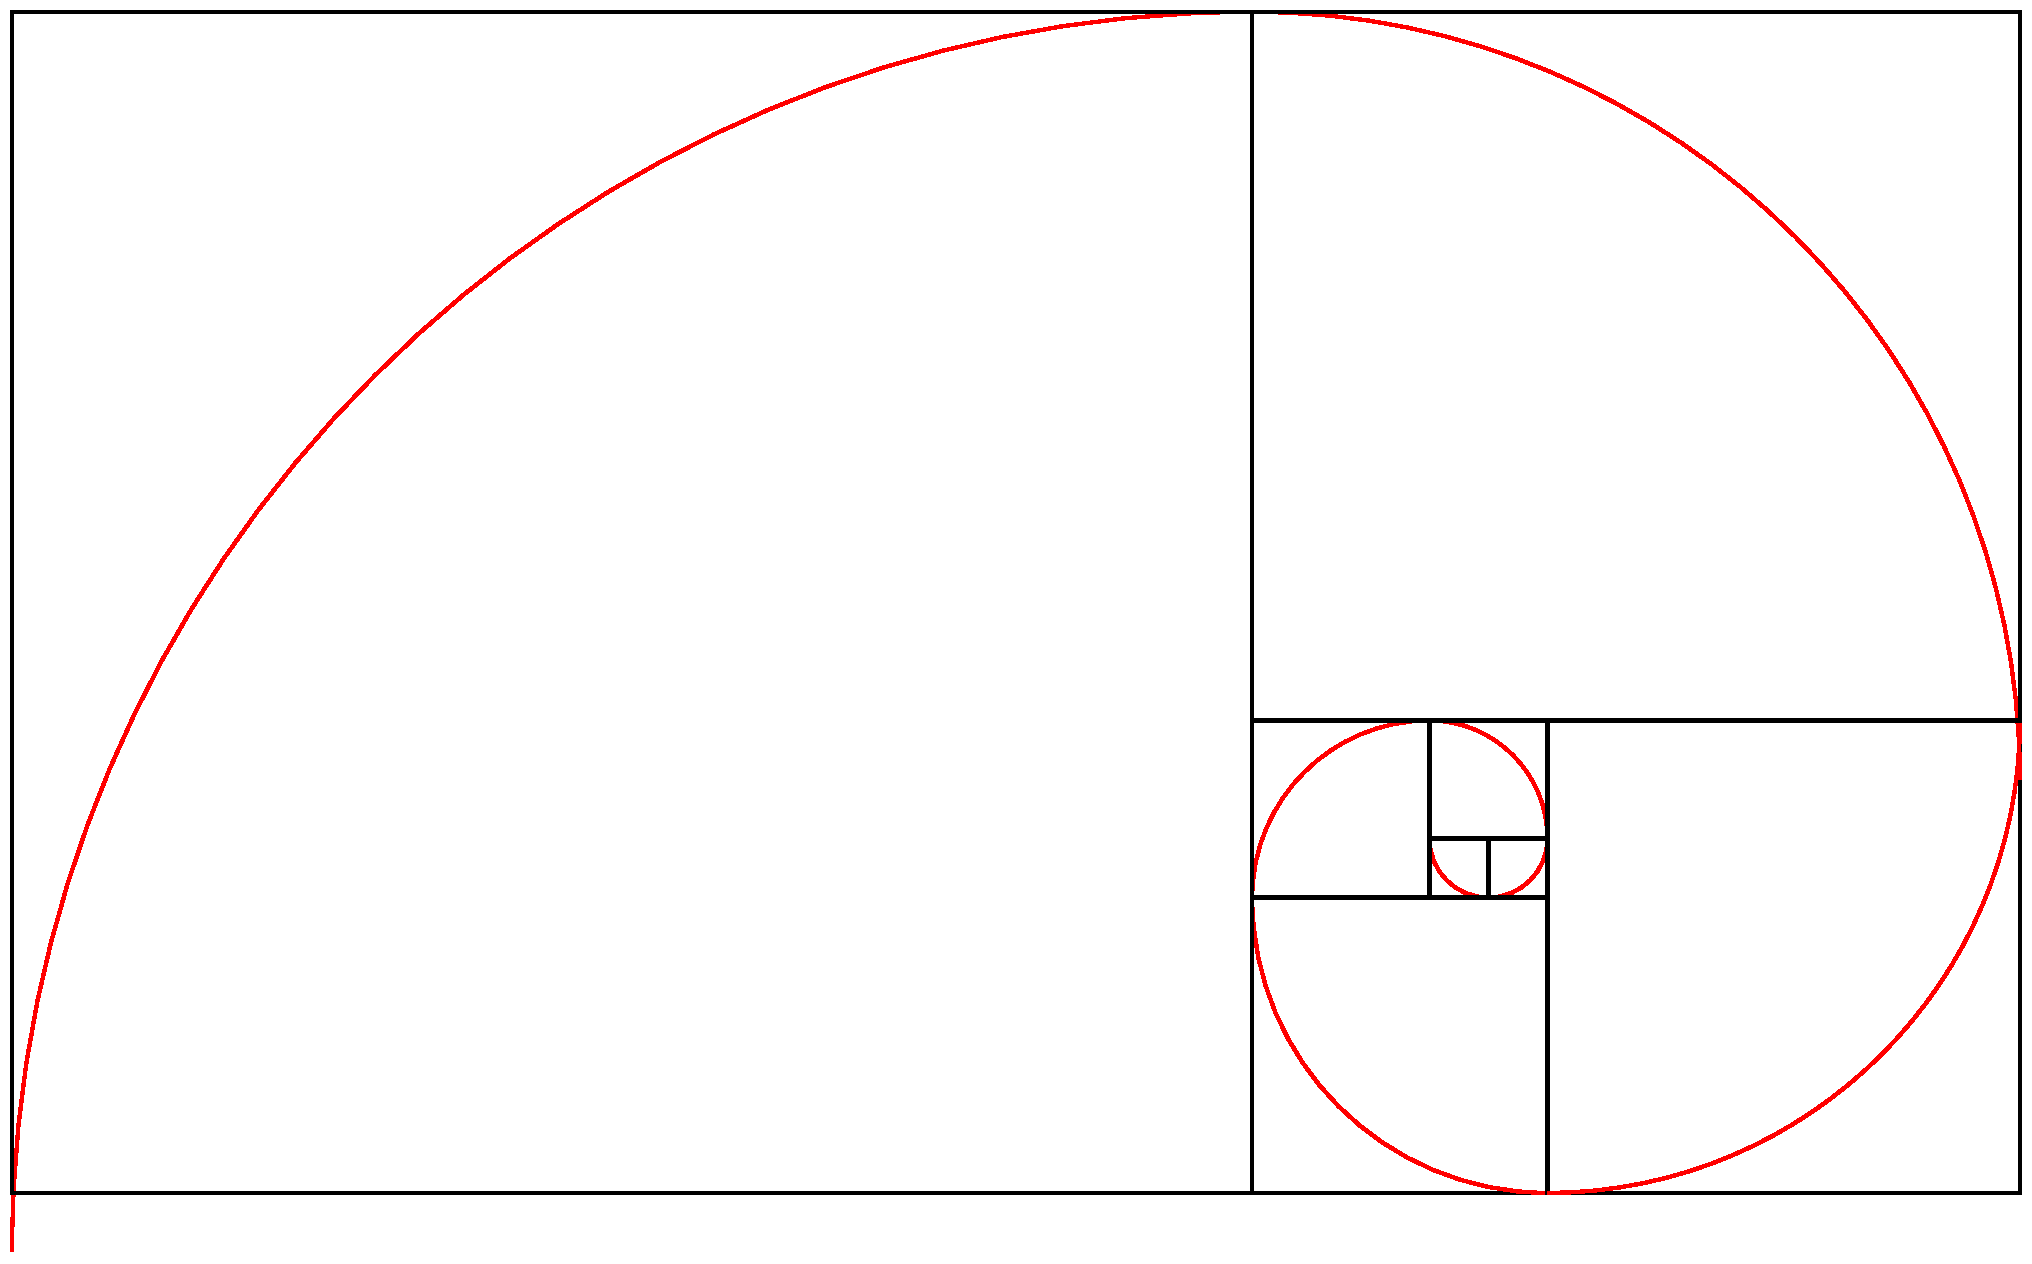
\includegraphics[height=4cm]{target-08-figure}
\end{minipagex}

\nopagebreak

\fbox{\phantom{ANSWER}}~ways

\begin{answer}
\begin{tikzpicture}\node[textbox]{%
    \begin{minipagex}{\dimexpr\textwidth-20pt}
        TO DO: COPY MY NOTES
        \begin{empheq}[box={\mathbox[colback=white]}]{equation*}
            96 ~\text{ways}
        \end{empheq} 
    \end{minipagex}
    };
\end{tikzpicture}%
\end{answer}
%%%%%%%%%%%%%%%%%%%%%%%%%%%%%%%%%%%%%%%%%%%%%%%%%%%%%%%%%%%%%%%%%%%%%%%%


\end{document}